% This is samplepaper.tex, a sample chapter demonstrating the
% LLNCS macro package for Springer Computer Science proceedings;
% Version 2.21 of 2022/01/12
%
\documentclass[runningheads]{llncs}
%
\usepackage[T1]{fontenc}
\usepackage[vietnamese]{babel} % Nhớ bỏ cái này đi sau khi nháp xong
% T1 fonts will be used to generate the final print and online PDFs,
% so please use T1 fonts in your manuscript whenever possible.
% Other font encondings may result in incorrect characters.
%
\usepackage{graphicx}
% Used for displaying a sample figure. If possible, figure files should
% be included in EPS format.
%
% If you use the hyperref package, please uncomment the following two lines
% to display URLs in blue roman font according to Springer's eBook style:
%\usepackage{color}
%\renewcommand\UrlFont{\color{blue}\rmfamily}
%\urlstyle{rm}
%
\begin{document}
%
\title{Genetic Algorithm Optimization Techniques for Steiner Problem in Graph}
%
%\titlerunning{Abbreviated paper title}
% If the paper title is too long for the running head, you can set
% an abbreviated paper title here
%

\author{Phu-Quy Le-Tang \and
Dai-Tho Dang \and
Bao-Nhan Ho-Sy \and
Phu-Quoc Hoang-Tan
}
%
\authorrunning{L.T.P.Quy et al.}
% First names are abbreviated in the running head.
% If there are more than two authors, 'et al.' is used.
%
\institute{VKU University, Princeton NJ 08544, USA\\
\email{\{quyltp.22git,quochtp.22git,nhanhsb.22git,thay Tho\}@vku.udn.vn}}
% \email{lncs@springer.com}\\
% \url{http://www.springer.com/gp/computer-science/lncs} \and
% ABC Institute, Rupert-Karls-University Heidelberg, Heidelberg, Germany\\
% \email{\{abc,lncs\}@uni-heidelberg.de}}
%
\maketitle              % typeset the header of the contribution
%
\begin{abstract}
    Steiner Tree Problem in Graph is a NP-Hard problem gathered much attention worldwide. 
    Genetic Algorithm is a simple yet efficient meta-heuristic optimizer that has been adopted in wide range of NP class problems. 
    In this paper, we investigated the efficiency of different diversity preservation techniques for GA in the context of SPG. 
    By using a fast implementation of bit string representation, appropriate searching operator, 
    we achieved a high-performance algorithm with low time cost. The algorithm is seperated into small version, where techniques 
    are incrementally added: Elitism Selection, Longest Distance elements, Dynamic Crossover Rate, Fitness Sharing, and an explicit
    population control procedure "Divergence".

\keywords{Steiner tree problem in graph  \and Genetic algorithm \and Another keyword.}
\end{abstract}
%
%
%
\section{TEAM DISCUSSION}
Dặn dò chung: Nguyên tắc khi viết một bài báo NCKH là:
- "Liêm chính khoa học"

Tức là những ý tưởng gì hay công trình đã có trước đó mà mình nhắc lại, mượn lại, sử dụng (cho dù vô tình), 
thì đều phải trích dẫn đàng hoàng (vào file .bib)

Quý sẽ chém gió phần thuật toán (methodology, approach, ...) vì Quý ôm làm hết mất :D. 
Anh em phụ phần khác. Đặc biệt rất cần anh em viết giúp được luôn phần Experimental

Experiment: Mình lấy mấy bộ test chạy để generate ra kết quả, xong từ kết quả phân tích số liệu, thống kê theo các phương pháp khoa học để 
\textbf{chứng minh} một nhận định nào đó của bản thân.

Quý sẽ đưa kết luận trước còn đọc số liệu thì tin tưởng giao anh em nhá. Kết quả thì chạy sắp xong rồi

Hồi đi học, gặp lại sẽ thảo luận, chỉ dẫn rõ là cần include vào những bảng, figure gì và cần phân tích như thế nào.

\section{Introduction}
Phần này lấn luôn cả Related Work

// Quốc \& Nhân chia nhau section này

\subsection{Intro SPG}
Introduction about SPG: Its hardness, wide-range application, gathered lots of interest around the world.
 
\begin{itemize}
    \item SPG is NP-Hard
    \item Application: Phải nói được có hai bài toán khác nhau (coi sách Advances in Steiner Tree):
        + geometric Steiner Tree problem: Cho trước một tập điểm trong mặt phẳng, không gian, ..., với đơn vị khoảng cách là Manhattan hay Euclid
        có thể tìm thêm một vài điểm trung gian (gọi là Steiner) để kết nối tập Terminal cho trước với tổng chi phí nhỏ nhất
        như là VLSI
        + STP in graph (SPG): là cái mình đang giải. Tới năm 2011 nó có nhiều variants rồi (https://dimacs11.zib.de/downloads.html),
        nhưng mà mình vẫn giải dạng kinh điển nhất.
    \item Trích dẫn một số State-of-the-art results, những hướng tiếp cận của người ta (cứ tham khảo như của trong anh Chương)
\end{itemize}

\subsubsection{Problem Formulation}

Phát biểu bằng công thức toán bài toán SPG

\subsection{Intro GA}
Intro GA: Simplicity, efficiency, examples of applying GA for SPG.
    
Sơ lược về lịch sử (John Holland 1975), 
    
    ứng dụng rộng rãi trong các bài toán hiệu quả như thế nào,

    ý tưởng sơ lược \& chung nhất của GA (Introduction to Evolutionary Algorithms),

    các thảo luận trước đó "in literature" về việc duy trì diversity, cân bằng giữa exploration và exploitation (AEGA),  

\subsubsection{Application of GA in Steiner Tree}

    Chắc tìm trên GG Scholar. Phần này viết giống Related Work. Ông nào làm gì thì tóm tắt cách làm của ông trong 1-2 câu rồi Cite.

    Lấy hai bài của người Việt mình, một bài của team BKHN nè (bài còn lại được trích trong đấy).


\section{Hai section tiếp theo đây là phần sân của Quý}
Note: chú ý nhớ tìm cite cho cẩn thận vì hình như Q toàn nghĩ ra ý tưởng mấy ông làm vài chục năm trước ròi.
% \section{Solution representation and Genetic searching operators}
\section{Genetic Algorithm preliminaries}
\subsection{Solution Representation}
Nghiệm nhị phân. Dùng chuỗi số nguyên 64 bit để biểu diễn các bit nhị phân.
So sánh với cách biểu diễn theo đỉnh như của Kapsalis hay ông gì đó xưa từ 90(s)
Ưu điểm: 
- Do cách cài đặt này nên các thao tác được nhanh, độ phức tạp O(max(số lượng bit 1 bật, |E| / 64)) = O(max(|V|, |E| / 64))
- Không gian biểu diễn bao trùm toàn bộ không gian nghiệm

Nhược điểm: Không gian tìm kiếm quá rộng và quá nhiều chỗ bị invalid.

\subsection{Self-correcting operators}
- Reduce: cắt bớt cạnh thừa
- Make Span: kết nối các thành phần không liên thông lại với nhau bằng đường đi ngắn nhất

\subsection{Crossover \& Mutation}
- Theo code + sơ đồ mà chém

\subsection{Randomized Data Structure}
- Shortest Path Floyd
- Almost MST

\section{Proposed Metaheuristics Algorithms}
\subsection{"Simple" GA}
SGA. Viết pseudo code thuật toán. Cite CHC Adaptive Search. Giải thích na ná như vậy.

\subsection{"Regular" GA}
Giải thích những phần thêm so với SGA. (SGA + 2 Elitist and 3 Longest Distance for each + Augment)

\subsection{IGA or IGA\_F}
Chém gió gì đấy tiếp

\subsection{Reduction Test}
In STP literature, pre-processing is the most vital and effective procedure for almost any approaches, 
while consumes relatively low time compared to the main solver.

In this approach, we adopt 2 simple reduction tests: Shortest-Distance Test and Degree-Test (cite KM96)

\section{Experimental Results}
\subsection{Set-up}
LƯU Ý: Chạy ra 2 kết quả: với bộ input đã rút gọn và bộ input gốc.

Tham khảo nhóm BKHN viết khá sướng mà hơi căng thẳng, nhiều kiến thức hiếm quá.

Chúng tôi sử dụng các testset $\dots$ từ SteinLib (cite) để benchmark. Cấu hình máy là $\dots$ Vì kết quả biến thiên tương đối lớn 
nên mỗi test đều được chạy 50 lần với mỗi thuật toán rồi average.

Metric: Độ lệch trung bình? Độ lệch max? Chắc hỏi thầy thêm.

\subsection{Result}
\subsection{Analysis}
Có thể viết liền mạch hai mục này ko cần tách ra subsection

Show ra một vài bảng (Bảng gì? Cần họp thêm)

Nhìn vào bảng ta thấy SGA chạy nhanh nhất, thời gian 3 thằng còn lại tương đương nhau.
Kết quả của thằng IGA\_F đối với series i080 và i160 thấp (tốt), $\dots$ hả.

Phân tích behavior: những thằng nào dễ rơi vào local (dựa vào log mà Quý chém). Những test nào khó. Những test nào kết quả chạy ra
có chênh lệch nhiều? Ví dụ chạy p465 có test xuống 3880 sát nút, có test thì 5000. 

\section{Conclusion}
Chém gió + một số hướng đi tương lai:
- Phần mềm minh họa demo
- Ứng dụng vào bài toán mạng truyền thông
- Kết hợp với góc nhìn + cách làm của những ông exact solver để nâng cao hiệu quả hơn nữa.

\section{Template}
\subsubsection{Sample Heading (Third Level)} Only two levels of
headings should be numbered. Lower level headings remain unnumbered;
they are formatted as run-in headings.

\paragraph{Sample Heading (Fourth Level)}
The contribution should contain no more than four levels of
headings. Table~\ref{tab1} gives a summary of all heading levels.

\begin{table}
\caption{Table captions should be placed above the
tables.}\label{tab1}
\begin{tabular}{|l|l|l|}
\hline
Heading level &  Example & Font size and style\\
\hline
Title (centered) &  {\Large\bfseries Lecture Notes} & 14 point, bold\\
1st-level heading &  {\large\bfseries 1 Introduction} & 12 point, bold\\
2nd-level heading & {\bfseries 2.1 Printing Area} & 10 point, bold\\
3rd-level heading & {\bfseries Run-in Heading in Bold.} Text follows & 10 point, bold\\
4th-level heading & {\itshape Lowest Level Heading.} Text follows & 10 point, italic\\
\hline
\end{tabular}
\end{table}


\noindent Displayed equations are centered and set on a separate
line.
\begin{equation}
x + y = z
\end{equation}
Please try to avoid rasterized images for line-art diagrams and
schemas. Whenever possible, use vector graphics instead (see
Fig.~\ref{fig1}).

\begin{figure}
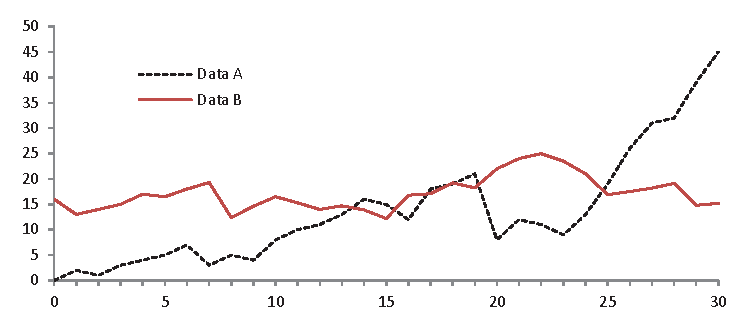
\includegraphics[width=\textwidth]{fig1.eps}
\caption{A figure caption is always placed below the illustration.
Please note that short captions are centered, while long ones are
justified by the macro package automatically.} \label{fig1}
\end{figure}

\begin{theorem}
This is a sample theorem. The run-in heading is set in bold, while
the following text appears in italics. Definitions, lemmas,
propositions, and corollaries are styled the same way.
\end{theorem}
%
% the environments 'definition', 'lemma', 'proposition', 'corollary',
% 'remark', and 'example' are defined in the LLNCS documentclass as well.
%
\begin{proof}
Proofs, examples, and remarks have the initial word in italics,
while the following text appears in normal font.
\end{proof}
For citations of references, we prefer the use of square brackets
and consecutive numbers. Citations using labels or the author/year
convention are also acceptable. The following bibliography provides
a sample reference list with entries for journal
articles~\cite{ref_article1}, an LNCS chapter~\cite{ref_lncs1}, a
book~\cite{ref_book1}, proceedings without editors~\cite{ref_proc1},
and a homepage~\cite{ref_url1}. Multiple citations are grouped
\cite{ref_article1,ref_lncs1,ref_book1},
\cite{ref_article1,ref_book1,ref_proc1,ref_url1}.

\begin{credits}
\subsubsection{\ackname} A bold run-in heading in small font size at the end of the paper is
used for general acknowledgments, for example: This study was funded
by X (grant number Y).

\subsubsection{\discintname}
It is now necessary to declare any competing interests or to specifically
state that the authors have no competing interests. Please place the
statement with a bold run-in heading in small font size beneath the
(optional) acknowledgments\footnote{If EquinOCS, our proceedings submission
system, is used, then the disclaimer can be provided directly in the system.},
for example: The authors have no competing interests to declare that are
relevant to the content of this article. Or: Author A has received research
grants from Company W. Author B has received a speaker honorarium from
Company X and owns stock in Company Y. Author C is a member of committee Z.
\end{credits}
%
% ---- Bibliography ----
%
% BibTeX users should specify bibliography style 'splncs04'.
% References will then be sorted and formatted in the correct style.
%
% \bibliographystyle{splncs04}
% \bibliography{mybibliography}
%
\begin{thebibliography}{8}
\bibitem{ref_article1}
Author, F.: Article title. Journal \textbf{2}(5), 99--110 (2016)

\bibitem{ref_lncs1}
Author, F., Author, S.: Title of a proceedings paper. In: Editor,
F., Editor, S. (eds.) CONFERENCE 2016, LNCS, vol. 9999, pp. 1--13.
Springer, Heidelberg (2016). \doi{10.10007/1234567890}

\bibitem{ref_book1}
Author, F., Author, S., Author, T.: Book title. 2nd edn. Publisher,
Location (1999)

\bibitem{ref_proc1}
Author, A.-B.: Contribution title. In: 9th International Proceedings
on Proceedings, pp. 1--2. Publisher, Location (2010)

\bibitem{ref_url1}
LNCS Homepage, \url{http://www.springer.com/lncs}, last accessed 2023/10/25
\end{thebibliography}
\end{document}
